% !TeX program = pdflatex
%==============================================================================
%  Aula 02 --- Regressão Linear e Regularização
%  VERSÃO DO ALUNO: texto para leitura autônoma, fora da sala.
%  (O roteiro de sala correspondente é "02 Regressao Linear e Regularizacao.tex".)
%
%  A figura da geometria l1/l2 é desenhada em TikZ com os valores EXATOS de um
%  ajuste real (n=60, duas covariáveis com correlação -0,50). Ver o comentário
%  imediatamente antes dela para os números e como reproduzi-los.
%==============================================================================
\documentclass[11pt,a4paper]{article}
\usepackage[aluno]{../../recursos/latex/estilo-notas}

\title{}
\date{}

\begin{document}
\cabecalhoaula{02}{Regressão Linear e Regularização}{AME cap.~2--3; ISLP cap.~3 e~6}

%==============================================================================
\section*{O que você vai aprender}
%==============================================================================
Ao final desta aula você deve ser capaz de:
\begin{itemize}[leftmargin=1.4cm]
  \item escrever o modelo de regressão linear em forma matricial e deduzir o
        estimador de mínimos quadrados (MQO);
  \item explicar por que MQO falha (ou nem existe) em \emph{altas dimensões}
        ($d$ grande, ou $d>n$);
  \item descrever seleção de subconjuntos e regressão \emph{stepwise};
  \item definir as penalizações \textbf{Ridge} ($\ell_2$) e \textbf{Lasso}
        ($\ell_1$) e interpretá-las como controle do balanço viés--variância;
  \item explicar \emph{por que o Lasso zera coeficientes} (esparsidade) e o Ridge
        não, com a intuição geométrica;
  \item reconhecer a interpretação bayesiana das duas penalizações.
\end{itemize}

\noindent
Esta aula é a Aula~01 em ação. Lá vimos que existe um balanço viés--variância e que
escolher um modelo é escolher um ponto nesse balanço. Aqui aprendemos a
\emph{mover esse ponto de propósito}, sem trocar de família de modelos: a
regularização introduz viés deliberadamente para comprar uma redução maior de
variância. Comece pela pergunta que motiva tudo:

\begin{center}\itshape
  se eu tenho 50 covariáveis e 30 observações, o que acontece com os mínimos
  quadrados?
\end{center}

\noindent
A resposta curta é ``algo pior do que dar errado: ele dá \emph{infinitas} respostas,
todas com erro de treino zero''. A Seção~\ref{sec:altadim} explica por quê.

%==============================================================================
\section{O modelo de regressão linear}
%==============================================================================
Métodos \textbf{paramétricos} supõem que a função de predição é descrita por um
número finito de parâmetros. A regressão linear usa
\begin{equation}\label{eq:linear}
  g(\x) = \bbeta^\top \x = \beta_0 x_0 + \beta_1 x_1 + \dots + \beta_d x_d,
  \qquad x_0 \equiv 1,
\end{equation}
com $\bbeta=(\beta_0,\dots,\beta_d)$. É essencial notar que $x_j$ \emph{não} precisa
ser uma covariável original: podemos criar atributos derivados ($x_j^2$, $x_jx_k$,
$\log x_j$, etc.). Assim, ``linear'' refere-se à linearidade \textbf{nos
parâmetros} $\bbeta$, não nas variáveis --- o modelo é muito mais flexível do que
parece à primeira vista.

\begin{ideia}
Você já usou isso na Aula~01 sem perceber. Ajustar um polinômio de grau~15 é
ajustar uma \emph{regressão linear} nas covariáveis $x,x^2,\dots,x^{15}$. Tudo o que
dissermos aqui sobre ``muitas covariáveis'' vale, portanto, também para ``polinômio
de grau alto''.
\end{ideia}

\subsection{Mínimos quadrados ordinários (MQO)}
Estimamos $\bbeta$ minimizando a soma dos quadrados dos resíduos (RSS):
\begin{equation}\label{eq:mqo}
  \widehat{\bbeta}
   = \argmin_{\bbeta} \sum_{i=1}^n
     \big(Y_i - \bbeta^\top \X_i\big)^2
   = \argmin_{\bbeta} \norm{\bm{Y} - \bm{X}\bbeta}^2 ,
\end{equation}
onde $\bm{X}\in\R^{n\times(d+1)}$ é a matriz de delineamento (linha $i$ igual a
$\X_i^\top$, com a coluna de $1$s) e $\bm{Y}=(Y_1,\dots,Y_n)^\top$.

\begin{proposicao}[Equações normais]\label{prop:normal}
Se $\bm{X}^\top\bm{X}$ é invertível, o minimizador de \eqref{eq:mqo} é
\begin{equation}\label{eq:betahat}
  \widehat{\bbeta} = (\bm{X}^\top\bm{X})^{-1}\bm{X}^\top \bm{Y}.
\end{equation}
\end{proposicao}
\begin{proof}
Seja $S(\bbeta)=\norm{\bm{Y}-\bm{X}\bbeta}^2
=\bm{Y}^\top\bm{Y}-2\bbeta^\top\bm{X}^\top\bm{Y}+\bbeta^\top\bm{X}^\top\bm{X}\bbeta$.
O gradiente é $\nabla S(\bbeta)=-2\bm{X}^\top\bm{Y}+2\bm{X}^\top\bm{X}\bbeta$.
Igualando a zero obtêm-se as \emph{equações normais}
$\bm{X}^\top\bm{X}\,\bbeta=\bm{X}^\top\bm{Y}$; como a Hessiana
$2\bm{X}^\top\bm{X}$ é semidefinida positiva, o ponto crítico é mínimo. Se
$\bm{X}^\top\bm{X}$ é invertível, vale \eqref{eq:betahat}.
\end{proof}

\begin{observacao}
$\widehat{\bbeta}$ é o estimador de máxima verossimilhança sob o modelo
$Y_i = \bbeta^\top\X_i + \varepsilon_i$, com $\varepsilon_i\sim N(0,\sigma^2)$
i.i.d. A predição é $\rhat(\x)=\widehat{\bbeta}^\top\x$. Sob o modelo linear
correto, MQO é o melhor estimador linear não-viesado (Gauss--Markov).
\end{observacao}

\subsection{E quando a linearidade é falsa?}
Quase sempre é. Vale então perguntar o que o MQO estima quando $r(\x)$ \emph{não} é
linear --- e a resposta é tranquilizadora.

\begin{teorema}[MQO converge para o melhor preditor linear]\label{teo:oraculo}
Seja $\bbeta^*=\argmin_{\bbeta}\E\big[(Y-\bbeta^\top\X)^2\big]$ o
\textbf{melhor preditor linear} (o ``oráculo''), e suponha
$\Sigma=\E[\X\X^\top]$ bem definida. Então, quando $n\to\infty$,
\[
  \widehat{\bbeta} \;\xrightarrow{\ P\ }\; \bbeta^*
  \qquad\text{e}\qquad
  \risco\big(g_{\widehat{\bbeta}}\big) \;\xrightarrow{\ P\ }\; \risco\big(g_{\bbeta^*}\big).
\]
\end{teorema}
\begin{proof}[Esboço]
Minimizando $\E[(Y-\bbeta^\top\X)^2]$ obtém-se $\bbeta^*=\Sigma^{-1}\alpha$, com
$\alpha_j=\E[YX_j]$. O estimador se escreve na mesma forma,
$\widehat{\bbeta}=\widehat\Sigma^{-1}\widehat\alpha$, com
$\widehat\Sigma=n^{-1}\sum_i\X_i\X_i^\top$ e
$\widehat\alpha_j=n^{-1}\sum_i Y_iX_{i,j}$. Pela lei dos grandes números
$\widehat\Sigma\to\Sigma$ e $\widehat\alpha\to\alpha$; o teorema de Mann--Wald
transporta a convergência através da função contínua
$(\Sigma,\alpha)\mapsto\Sigma^{-1}\alpha$, e de novo através de
$\bbeta\mapsto \risco(g_{\bbeta})$.
\end{proof}

\begin{ideia}
Traduzindo: mesmo com o modelo ``errado'', o MQO acerta \emph{a melhor aproximação
linear possível} de $r$ --- a projeção de $Y$ no espaço gerado pelas covariáveis. O
viés que sobra não é culpa do estimador, é culpa da classe de modelos escolhida.
Por isso ampliar o conjunto de atributos (incluir $x^2$, interações) reduz esse viés
de especificação --- ao custo de aumentar $d$, que é exatamente o problema da próxima
seção.
\end{ideia}

%==============================================================================
\section{O problema das altas dimensões}\label{sec:altadim}
%==============================================================================
Quando $d$ é grande relativamente a $n$, o MQO sofre de três males:
\begin{enumerate}[leftmargin=1.6cm]
  \item \textbf{Variância alta.} Quanto mais parâmetros, maior $\Var(\widehat{\bbeta})$
        --- o modelo superajusta (Aula~01). A matriz $\Var(\widehat{\bbeta})
        =\sigma^2(\bm{X}^\top\bm{X})^{-1}$ ``explode'' quando as colunas de
        $\bm{X}$ são quase colineares.
  \item \textbf{Não unicidade.} Se $d>n$, então $\bm{X}^\top\bm{X}$ é singular e
        \eqref{eq:betahat} \emph{não tem solução única}: há infinitos $\bbeta$ com
        RSS nulo (superajuste perfeito).
  \item \textbf{Interpretabilidade.} Muitas covariáveis irrelevantes dificultam a
        leitura do modelo.
\end{enumerate}

Vale ver o primeiro mal acontecer. Fixe $n=60$ observações e vá aumentando $d$, com
apenas 5 covariáveis de fato relevantes e o resto puro ruído
(Figura~\ref{fig:altadim}).

\begin{figure}[htbp]
  \centering
  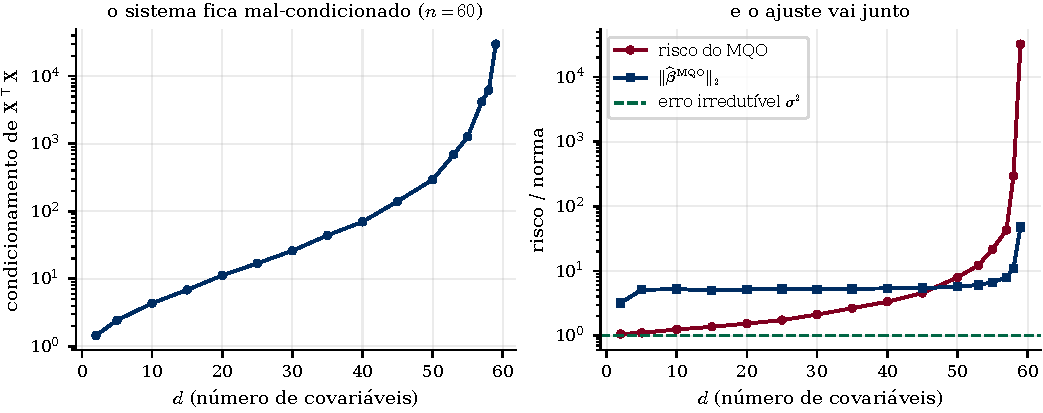
\includegraphics[width=\textwidth]{../../recursos/figuras/02-mqo-alta-dim.pdf}
  \caption{Com $n=60$ fixo e $d$ crescendo. À esquerda, o número de condição de
  $\bm{X}^\top\bm{X}$ --- a razão entre seu maior e seu menor autovalor --- sai de
  $1{,}4$ e chega a $3\times10^4$: inverter essa matriz vira uma operação
  numericamente delicada. À direita, a consequência: o risco do MQO sai de $1{,}0$
  (o próprio $\sigma^2$, ou seja, praticamente perfeito) e passa de $10^4$. O modelo
  não ficou ``um pouco pior''; ele ficou inútil.}
  \label{fig:altadim}
\end{figure}

\begin{atencao}[o caso $d>n$ é qualitativamente diferente]
Repare que os problemas 1 e 2 não são o mesmo. Se $d<n$ mas as colunas são quase
colineares, a solução \emph{existe e é única}, só que instável. Se $d>n$, ela nem é
única: o núcleo de $\bm{X}$ tem dimensão $\ge d-n$, e somar a $\widehat{\bbeta}$
qualquer vetor desse núcleo dá \emph{outra} solução com exatamente o mesmo RSS
nulo. O erro de treino não distingue entre elas, e não há nada nos dados que
justifique preferir uma. A regularização, entre outras coisas, serve para desempatar.
\end{atencao}

A resposta é \textbf{reduzir a complexidade efetiva}: ou selecionando um
subconjunto de covariáveis, ou \emph{encolhendo} os coeficientes (regularização).

\subsection{Seleção de subconjuntos e \emph{stepwise}}
\begin{description}[leftmargin=2.4cm,style=nextline]
  \item[Melhor subconjunto] ajusta-se o modelo para \emph{todos} os $2^d$
        subconjuntos de covariáveis e escolhe-se o melhor segundo um critério que
        penaliza complexidade (AIC, BIC) ou via validação cruzada. Inviável para
        $d$ moderado ($2^d$ explode).
  \item[\emph{Forward stepwise}] começa com o modelo vazio e adiciona, a cada
        passo, a covariável que mais reduz o RSS, até um critério de parada.
  \item[\emph{Backward stepwise}] começa com o modelo completo e remove, a cada
        passo, a covariável menos útil (exige $n>d$).
\end{description}

A economia do \emph{stepwise} é enorme: ele examina $1+d(d+1)/2$ modelos em vez de
$2^d$. Para $d=20$ isso é $211$ contra $1\,048\,576$; para $d=40$, $821$ contra
mais de $10^{12}$.

\begin{exemplo}[Quanto isso custa, na prática]\label{ex:ame31}
O [AME] simula $n=500$ observações de
$Y = 3X_1-2X_2+X_3-3X_4+X_5+\sum_{i=6}^{20}0\cdot X_i+\varepsilon$, com
$\varepsilon\sim N(0;0{,}5^2)$: apenas 5 das 20 covariáveis importam. Os resultados:
\begin{center}\small
\renewcommand{\arraystretch}{1.2}
\begin{tabular}{@{}llrl@{}}
\toprule
\textbf{Método} & \textbf{Variáveis selecionadas} & \textbf{Tempo} & \textbf{Risco estimado} \\
\midrule
Mín.\ quadrados      & todas                    & 0,002 s & 14,63 \\
Melhor subconj.\ (AIC) & $x_1..x_5,x_{10},x_{12},x_{13},x_{19},x_{20}$ & 1 h 20 min & 0,30 \\
\emph{Forward stepwise}  & $x_1..x_5,x_{10},x_{12},x_{13},x_{19},x_{20}$ & 0,46 s & 0,30 \\
Ridge                & todas                    & 0,16 s & 0,33 \\
Lasso                & $x_1,\dots,x_5$          & 0,08 s & \textbf{0,25} \\
\bottomrule
\end{tabular}
\end{center}
Três leituras. Primeira: o MQO com todas as variáveis tem risco \emph{cinquenta
vezes} maior que o Lasso --- as 15 covariáveis nulas destroem o modelo. Segunda: o
\emph{forward stepwise} encontrou exatamente o mesmo modelo do melhor subconjunto
em $0{,}46$ segundos em vez de $1$h$20$; a heurística gananciosa saiu de graça aqui.
Terceira: o Lasso foi o mais rápido \emph{e} o único a recuperar precisamente
$\{x_1,\dots,x_5\}$.
\end{exemplo}

\begin{atencao}
Critérios como AIC/BIC ($\riscohat \approx \mathrm{EQM} + P(g)$, com
$P(g)\propto p/\widehat\sigma^2$) estimam o risco \emph{corrigindo} o otimismo do
erro de treino. Mas seleção \emph{stepwise} é gananciosa (não examina todos os
modelos) e a inferência clássica ``pós-seleção'' fica inválida: os $p$-valores
reportados ignoram que o modelo foi escolhido olhando os dados. Um $p$-valor de
$0{,}01$ numa variável que sobreviveu a uma triagem entre 20 candidatas não
significa o que a tabela diz que significa.
\end{atencao}

%==============================================================================
\section{Regularização: encolhendo coeficientes}
%==============================================================================
A ideia da regularização (ou \emph{penalização}, ou \emph{shrinkage}) é adicionar
ao RSS um termo que penaliza coeficientes grandes, desencorajando o superajuste:
\[
  \widehat{\bbeta}_{\text{pen}}
  = \argmin_{\bbeta}\Big\{ \norm{\bm{Y}-\bm{X}\bbeta}^2
       + \lambda\, \mathrm{Pen}(\bbeta) \Big\}.
\]
O hiperparâmetro $\lambda\ge 0$ controla a intensidade: $\lambda=0$ recupera MQO;
$\lambda\to\infty$ força $\bbeta\to 0$. \textbf{$\lambda$ é escolhido por validação
cruzada} (Aula~03).

\begin{ideia}
Regularizar = introduzir \emph{viés} de propósito para reduzir \emph{variância}.
Sob $d$ grande, o ganho na variância supera a perda no viés e o risco total cai.
É a Aula~01 em ação.
\end{ideia}

\subsection{Qual medida de complexidade?}
Antes das fórmulas, vale escolher \emph{como medir} o tamanho de $\bbeta$. Há três
candidatas naturais, e a comparação entre elas explica por que o Lasso é o que é:
\begin{center}\small
\renewcommand{\arraystretch}{1.25}
\begin{tabular}{@{}lccc@{}}
\toprule
$\bbeta$ (com $d=10$) & $\sum_j\1{\beta_j\neq0}$ ($\ell_0$)
                      & $\sum_j\abs{\beta_j}$ ($\ell_1$)
                      & $\sum_j\beta_j^2$ ($\ell_2$) \\
\midrule
$(0,0,\dots,0)$              & $0$  & $0{,}0$  & $0$  \\
$(0{,}1;0{,}1;\dots;0{,}1)$  & $10$ & $1{,}0$  & $0{,}1$ \\
$(1,1,\dots,1)$              & $10$ & $10{,}0$ & $10$ \\
\bottomrule
\end{tabular}
\end{center}
Compare as linhas 1 e 2: os dois modelos fazem predições quase idênticas, mas a
norma $\ell_0$ salta de $0$ para $10$ --- ela é \emph{descontínua}, uma mudança
infinitesimal nos coeficientes muda a penalização ao máximo. Compare agora as linhas
2 e 3: as predições são \emph{muito} diferentes, e ainda assim a $\ell_0$ dá o mesmo
valor $10$ para as duas. A norma $\ell_0$ é, ao mesmo tempo, sensível demais e
insensível demais.

\begin{ideia}
A norma $\ell_1$ é o melhor dos dois mundos: como a $\ell_0$, ela é pequena para
vetores com muitos zeros --- e por isso induz esparsidade; ao contrário da $\ell_0$,
ela varia \emph{continuamente} com $\bbeta$, o que torna o problema convexo e
resolúvel em milissegundos. Não é exagero dizer que o Lasso existe porque a $\ell_1$
é a relaxação convexa da $\ell_0$.
\end{ideia}

\subsection{Regressão Ridge ($\ell_2$)}
\begin{equation}\label{eq:ridge}
  \widehat{\bbeta}^{\,\text{ridge}}
   = \argmin_{\bbeta}\Big\{ \norm{\bm{Y}-\bm{X}\bbeta}^2
       + \lambda \sum_{j=1}^{d}\beta_j^2 \Big\}.
\end{equation}
A grande vantagem é a solução fechada:
\begin{equation}\label{eq:ridgesol}
  \widehat{\bbeta}^{\,\text{ridge}}
   = (\bm{X}^\top\bm{X} + \lambda \bm{I}_0)^{-1}\bm{X}^\top\bm{Y},
\end{equation}
onde $\bm{I}_0$ é a identidade $(d+1)\times(d+1)$ \emph{com o primeiro elemento
trocado por zero} --- é assim que se deixa o intercepto $\beta_0$ fora da
penalização. (Faz sentido: penalizar $\beta_0$ tornaria a solução dependente de onde
você pôs a origem de $Y$.)

\begin{proposicao}[Ridge sempre tem solução única]
Para todo $\lambda>0$, a matriz $\bm{X}^\top\bm{X}+\lambda\bm{I}$ é definida
positiva (logo invertível), mesmo quando $d>n$.
\end{proposicao}
\begin{proof}
Para qualquer $\bm{v}\neq 0$,
$\bm{v}^\top(\bm{X}^\top\bm{X}+\lambda\bm{I})\bm{v}
=\norm{\bm{X}\bm{v}}^2+\lambda\norm{\bm{v}}^2\ge \lambda\norm{\bm{v}}^2>0$.
\end{proof}
Eis a primeira virtude do Ridge: \emph{estabiliza} o problema mal-condicionado das
altas dimensões. Note que a demonstração é exatamente o antídoto para a
Figura~\ref{fig:altadim}: somar $\lambda$ à diagonal levanta o menor autovalor de
$\bm{X}^\top\bm{X}$ de perto de zero para pelo menos $\lambda$, e o número de
condição desaba. Os coeficientes são encolhidos suavemente em direção a zero, mas
em geral \textbf{nenhum é exatamente zero}.

\subsection{O Lasso ($\ell_1$)}
\begin{equation}\label{eq:lasso}
  \widehat{\bbeta}^{\,\text{lasso}}
   = \argmin_{\bbeta}\Big\{ \norm{\bm{Y}-\bm{X}\bbeta}^2
       + \lambda \sum_{j=1}^{d}\abs{\beta_j} \Big\}.
\end{equation}
Trocamos a norma $\ell_2$ pela $\ell_1$. Não há solução fechada (o termo
$\abs{\beta_j}$ não é diferenciável em $0$), mas o problema é convexo e resolvido
eficientemente (\emph{coordinate descent}, LARS). A propriedade marcante:

\begin{ideia}
O Lasso faz \textbf{seleção de variáveis}: para $\lambda$ grande o suficiente,
vários $\widehat\beta_j$ são \emph{exatamente} zero. Obtemos um modelo
\emph{esparso} e interpretável de graça --- ao contrário do Ridge.
\end{ideia}

\begin{observacao}[Por que o Lasso aguenta $d$ enorme]
Greenshtein e Ritov (2004) mostram que, sob condições de limitação, o Lasso com
restrição $\norm{\bbeta}_1\le L$ satisfaz, com probabilidade $\ge 1-\delta$,
\[
  \risco(g_{\widehat{\bbeta}_L}) - \risco(g_{\bbeta^*_L})
  \;\le\; \sqrt{\frac{16(L+1)^4B^2}{n}\,\log\!\Big(\frac{2d}{\delta}\Big)} .
\]
O detalhe que importa é onde o $d$ aparece: dentro de um \textbf{logaritmo}. Dobrar
o número de covariáveis quase não muda a garantia --- é por isso que o Lasso funciona
com milhares de covariáveis e $n$ modesto, situação em que o MQO nem está definido.
\end{observacao}

\subsubsection*{Por que o Lasso zera coeficientes e o Ridge não?}
Ambos têm a formulação equivalente \emph{com restrição}: para cada $\lambda$ existe
um orçamento $t$ tal que resolver \eqref{eq:lasso} é o mesmo que resolver
\[
  \min_{\bbeta}\ \norm{\bm{Y}-\bm{X}\bbeta}^2
  \quad\text{sujeito a}\quad
  \underbrace{\textstyle\sum_j\abs{\beta_j}\le t}_{\text{Lasso}}
  \quad\text{ou}\quad
  \underbrace{\textstyle\sum_j\beta_j^2\le t^2}_{\text{Ridge}}.
\]
Nessa forma a geometria fica visível. As curvas de nível do RSS são
\emph{elipses} concêntricas centradas em $\widehat{\bbeta}^{\text{MQO}}$ --- e são
elipses \emph{alongadas} quando as covariáveis são correlacionadas, porque nessa
direção dá para aumentar um coeficiente e diminuir o outro quase sem alterar o
ajuste. A solução penalizada é o ponto onde a menor elipse possível \emph{toca} a
região permitida. E aí a forma da região decide tudo: a bola do Ridge é lisa, então o
contato se dá num ponto genérico; o losango do Lasso tem \emph{quinas sobre os
eixos}, e é muito fácil que o toque aconteça justamente numa quina --- onde algum
$\beta_j$ é exatamente zero.

% ---------------------------------------------------------------------------
% Figura da geometria. Números de um ajuste REAL, não desenhados no olho.
% Reproduzível com: n=60, duas covariáveis padronizadas com correlação -0,50,
% semente 13, beta verdadeiro (1,5 ; 0,55), ruído N(0,1).
%   beta_MQO = (1,573 ; 0,808)
%   Elipse do RSS: eixo MAIOR a 45 graus.
%   Lasso (alpha=0,65): (0,4846 ; 0) na quina; t1=0,4846;
%                       elipse tangente com semi-eixos (1,389 ; 0,757).
%   Ridge (alpha=20):   (1,0032 ; 0,3741);      t2=1,0706;
%                       elipse tangente com semi-eixos (0,731 ; 0,398).
% Conferido numericamente: a elipse tangente NÃO invade o losango (o mínimo do
% RSS sobre a borda coincide com o valor na solução) e a normal do RSS na quina
% cai a 18,5 graus, bem dentro do cone normal [-45,45] -- por isso o contato é
% um toque de frente na quina, e não um encosto na aresta.
% ---------------------------------------------------------------------------
\begin{figure}[htbp]
  \centering
  \begin{tikzpicture}[scale=1.42, >=Stealth]
    \foreach \dx in {0, 4.55} {
      \begin{scope}[shift={(\dx,0)}]
        \draw[->,gray!70] (-1.35,0) -- (2.85,0) node[right,black,font=\small] {$\beta_1$};
        \draw[->,gray!70] (0,-1.25) -- (0,2.05) node[above,black,font=\small] {$\beta_2$};
      \end{scope}
    }

    % ---------------- painel esquerdo: LASSO ----------------
    \begin{scope}
      \foreach \s in {0.32, 0.66} {
        \draw[verdeesc!50,thin,rotate around={45:(1.573,0.808)}]
          (1.573,0.808) ellipse [x radius={1.389*\s}, y radius={0.757*\s}];
      }
      \draw[verdeesc,thick,rotate around={45:(1.573,0.808)}]
        (1.573,0.808) ellipse [x radius=1.389, y radius=0.757];
      \fill[vinho!16] (0.4846,0) -- (0,0.4846) -- (-0.4846,0) -- (0,-0.4846) -- cycle;
      \draw[vinho,thick] (0.4846,0) -- (0,0.4846) -- (-0.4846,0) -- (0,-0.4846) -- cycle;
      \fill[black] (1.573,0.808) circle (1.3pt);
      \node[font=\scriptsize,right=2pt] at (1.573,0.808) {$\widehat{\bbeta}^{\text{MQO}}$};
      \fill[vinho] (0.4846,0) circle (1.9pt);
      \node[font=\scriptsize,vinho,below right=1pt and -3pt] at (0.4846,0) {$(0{,}48\,;\,\mathbf{0})$};
      \node[font=\small\bfseries,vinho] at (0.75,-1.45) {Lasso ($\ell_1$)};
    \end{scope}

    % ---------------- painel direito: RIDGE ----------------
    \begin{scope}[shift={(4.55,0)}]
      \foreach \s in {0.32, 0.66} {
        \draw[verdeesc!50,thin,rotate around={45:(1.573,0.808)}]
          (1.573,0.808) ellipse [x radius={0.731*\s}, y radius={0.398*\s}];
      }
      \draw[verdeesc,thick,rotate around={45:(1.573,0.808)}]
        (1.573,0.808) ellipse [x radius=0.731, y radius=0.398];
      \fill[azulufrj!13] (0,0) circle (1.0706);
      \draw[azulufrj,thick] (0,0) circle (1.0706);
      \fill[black] (1.573,0.808) circle (1.3pt);
      \node[font=\scriptsize,right=2pt] at (1.573,0.808) {$\widehat{\bbeta}^{\text{MQO}}$};
      \fill[azulufrj] (1.0032,0.3741) circle (1.9pt);
      \node[font=\scriptsize,azulufrj,right=3pt] at (1.0032,0.3741) {$(1{,}00\,;\,0{,}37)$};
      \node[font=\small\bfseries,azulufrj] at (0.75,-1.45) {Ridge ($\ell_2$)};
    \end{scope}
  \end{tikzpicture}
  \caption{A geometria da esparsidade, com números de um ajuste real ($n=60$, duas
  covariáveis padronizadas com correlação $-0{,}50$). Em verde, curvas de nível do
  RSS, centradas em $\widehat{\bbeta}^{\text{MQO}}=(1{,}573\,;\,0{,}808)$ e
  alongadas porque as covariáveis são correlacionadas. Em cor, a região permitida.
  A solução é o ponto onde a menor elipse \emph{toca} a região. À esquerda, o toque
  cai na \textbf{quina} do losango e $\beta_2$ sai exatamente zero; à direita, o
  círculo não tem quina, o toque acontece num ponto qualquer da borda e os dois
  coeficientes sobrevivem --- apenas encolhidos. Os orçamentos $t$ dos dois painéis
  são diferentes (cada método com o seu); o que se compara aqui é a \emph{forma} da
  região, não o seu tamanho.}
  \label{fig:geometria}
\end{figure}

\begin{atencao}
Perceba que a esparsidade do Lasso é um acidente \emph{feliz} da geometria, e não
uma regra infalível. Se a elipse estivesse orientada de outro jeito --- por exemplo,
se $\widehat{\bbeta}^{\text{MQO}}$ estivesse perto da diagonal ---, o toque cairia
numa aresta e nenhum coeficiente seria zerado. Em dimensão $d$, porém, o losango tem
$2d$ quinas e $2^d$ faces de dimensão baixa, e a chance de acertar alguma cresce
depressa. É por isso que ``o Lasso zera coeficientes'' é uma afirmação sobre o
comportamento \emph{típico}, não um teorema.
\end{atencao}

\begin{exemplo}[Caso ortonormal: fórmulas explícitas]
Quando $\bm{X}^\top\bm{X}=\bm{I}$, os estimadores têm forma fechada em função do
MQO $\widehat\beta_j$:
\[
  \widehat\beta_j^{\,\text{ridge}} = \frac{\widehat\beta_j}{1+\lambda},
  \qquad
  \widehat\beta_j^{\,\text{lasso}}
     = \operatorname{sinal}(\widehat\beta_j)\,\big(\abs{\widehat\beta_j}-\tfrac{\lambda}{2}\big)_+ .
\]
O Ridge \emph{multiplica} por um fator $<1$ (encolhe proporcionalmente, nunca
zera); o Lasso \emph{subtrai} uma constante e trunca em zero (\emph{soft
thresholding}) --- por isso anula os pequenos.
\end{exemplo}

\begin{figure}[htbp]
  \centering
  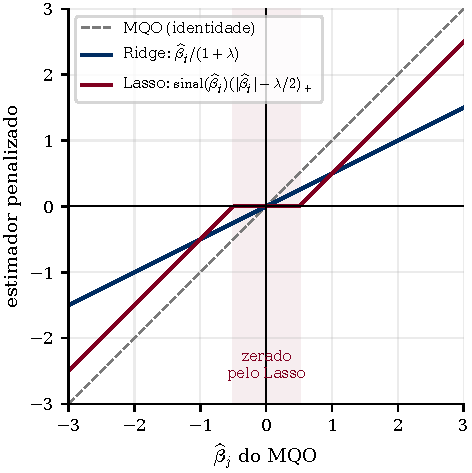
\includegraphics[width=0.56\textwidth]{../../recursos/figuras/02-soft-threshold.pdf}
  \caption{As duas fórmulas do caso ortonormal, com $\lambda=1$. O Ridge é uma reta
  pela origem de inclinação $1/(1+\lambda)$: encolhe \emph{proporcionalmente}, e
  quanto maior o coeficiente, maior o encolhimento em valor absoluto. O Lasso é
  paralelo à identidade, deslocado de $\lambda/2$: encolhe todo mundo pela
  \emph{mesma quantidade} --- e quem era menor que $\lambda/2$ em módulo (a faixa
  sombreada) não sobrevive ao deslocamento e vira exatamente zero.}
  \label{fig:soft}
\end{figure}

\subsection{Interpretação bayesiana}
Ambas as penalizações são o \emph{logaritmo de uma priori} sobre $\bbeta$. Suponha
$Y_i\mid\x_i,\bbeta\sim N(\bbeta^\top\x_i,\sigma^2)$ independentes, com $\sigma^2$
conhecido. Então:
\begin{itemize}[leftmargin=1.4cm]
  \item se $\bbeta\sim N(0,\sigma_\beta^2\bm{I})$, a \textbf{moda a posteriori} de
        $\bbeta$ é exatamente a solução Ridge \eqref{eq:ridge} com
        $\lambda=\sigma^2/\sigma_\beta^2$;
  \item se $\beta_1,\dots,\beta_d\stackrel{\text{i.i.d.}}{\sim}
        \mathrm{Laplace}(0,\tau_\beta)$, a moda a posteriori é exatamente a solução
        Lasso \eqref{eq:lasso} com $\lambda=\sigma^2\tau_\beta$.
\end{itemize}
A priori de Laplace é mais ``pontuda'' em zero e tem caudas mais pesadas: ela
favorece soluções com muitos coeficientes \emph{nulos} e alguns grandes --- exatamente
a esparsidade observada.

\begin{ideia}[uma leitura filosófica]
Sob essa ótica, $\lambda$ \emph{é} a priori: quanto menor a dispersão que você
atribui a $\bbeta$ a priori, maior o $\lambda$ e mais encolhidas as estimativas.
Escolher $\lambda$ por validação cruzada equivale, então, a \textbf{escolher a
distribuição a priori que prediz melhor} --- usar a maquinaria bayesiana como
motivação para estimadores melhores, sem necessariamente comprar a interpretação
subjetiva.
\end{ideia}

\begin{atencao}
Uma sutileza que o [ISLP] faz questão de registrar: no caso Ridge a solução é a moda
\emph{e} a média a posteriori. No caso Lasso ela é só a \textbf{moda} --- a média a
posteriori do Lasso \emph{não} é esparsa. A esparsidade é uma propriedade daquele
ponto específico da distribuição, não da distribuição inteira.
\end{atencao}

\begin{atencao}
Como as penalizações somam $\beta_j^2$ ou $\abs{\beta_j}$, elas \textbf{dependem da
escala} das covariáveis. \emph{Sempre padronize} (média 0, variância 1) antes de
aplicar Ridge/Lasso, caso contrário variáveis em unidades grandes são penalizadas
de menos. Repare que o MQO \emph{não} tem esse problema: trocar metros por
centímetros só divide o coeficiente por 100 e a predição fica igual. Com penalização
isso deixa de valer, porque o termo $\lambda\sum\beta_j^2$ enxerga a mudança. Isso
conecta diretamente com a Aula~07 (\emph{pipelines} e \texttt{StandardScaler}).
\end{atencao}

%==============================================================================
\section{Caminhos de regularização}
%==============================================================================
Como $\lambda$ varre $[0,\infty)$, cada $\widehat\beta_j$ traça uma curva. Pôr todas
num gráfico --- o \textbf{caminho de regularização} --- é a melhor forma de ver a
diferença entre os dois métodos de uma vez só (Figura~\ref{fig:caminhos}).

\begin{figure}[htbp]
  \centering
  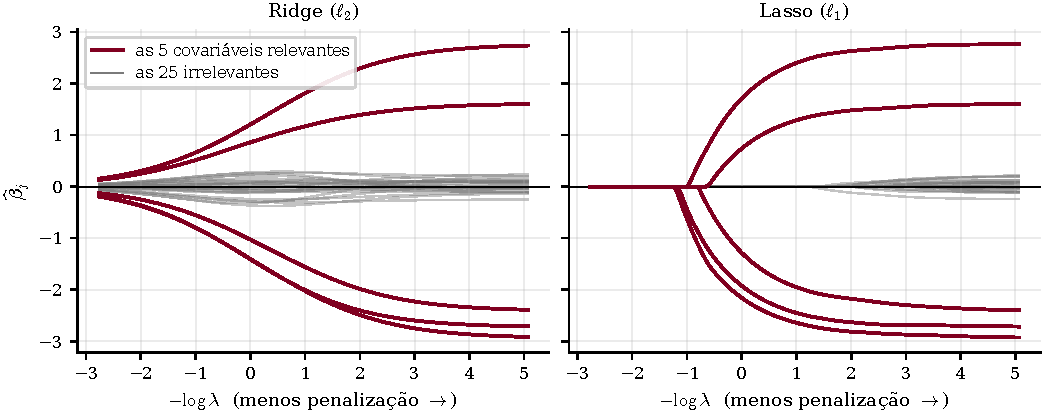
\includegraphics[width=\textwidth]{../../recursos/figuras/02-caminho-coeficientes.pdf}
  \caption{Coeficientes em função da penalização, num problema com $n=80$, $d=30$ e
  apenas 5 covariáveis relevantes. À esquerda o Ridge: todos os 30 coeficientes saem
  de zero \emph{juntos} e crescem suavemente --- em nenhum momento algum deles é
  exatamente nulo. À direita o Lasso: os coeficientes ficam \emph{grudados no zero} e
  vão sendo ``ligados'' um a um conforme a penalização afrouxa; as 5 covariáveis
  relevantes (em vinho) entram primeiro, muito antes das 25 irrelevantes (em cinza).
  É esse comportamento de liga-desliga que chamamos de seleção de variáveis.}
  \label{fig:caminhos}
\end{figure}

\begin{atencao}[o $\lambda$ que melhor prediz não é o que melhor seleciona]
Uma armadilha que aparece assim que você roda \texttt{LassoCV} num problema real: a
validação cruzada escolhe $\lambda$ para \emph{predizer} bem, e o $\lambda$ ótimo
para predição costuma ser \emph{menor} do que o ótimo para seleção. O resultado é um
modelo que prediz muito bem mas mantém coeficientes minúsculos e não nulos em várias
covariáveis irrelevantes --- falsos positivos. Se o seu objetivo é \emph{descobrir
quais} variáveis importam, e não só predizer, olhe o caminho inteiro e compare as
\emph{magnitudes}: as relevantes costumam estar ordens de grandeza acima do resto.
\end{atencao}

%==============================================================================
\section{Prática em Python}
%==============================================================================
Em \texttt{scikit-learn}, as três variantes seguem a mesma interface; o
\texttt{alpha} é o nosso $\lambda$. Note a padronização \emph{dentro} do
\emph{pipeline} (Aula~07) para evitar vazamento.
\begin{lstlisting}
from sklearn.linear_model import LinearRegression, Ridge, Lasso, LassoCV
from sklearn.preprocessing import StandardScaler
from sklearn.pipeline import make_pipeline

# Lasso com lambda escolhido por validacao cruzada
modelo = make_pipeline(StandardScaler(),
                       LassoCV(cv=5, random_state=0))
modelo.fit(X_tr, y_tr)

lasso = modelo.named_steps["lassocv"]
print("lambda escolhido:", lasso.alpha_)
print("coeficientes nao-nulos:", (lasso.coef_ != 0).sum(), "de", X.shape[1])
\end{lstlisting}

\begin{atencao}[um detalhe de escala que já custou caro a muita gente]
As classes do \texttt{scikit-learn} \textbf{não} usam a mesma normalização.
\texttt{Ridge} minimiza $\norm{y-\bm{X}\bbeta}^2+\alpha\norm{\bbeta}^2$, enquanto
\texttt{Lasso} e \texttt{ElasticNet} minimizam
$\tfrac{1}{2n}\norm{y-\bm{X}\bbeta}^2+\alpha\norm{\bbeta}_1$. Há um fator $n$ de
diferença: um $\alpha$ que é forte num é desprezível no outro. Ao comparar as duas
famílias na mesma grade, converta.
\end{atencao}

O notebook \texttt{Aula prática 02} percorre tudo isso com dados de verdade
(\texttt{superconductivity.csv}, $d=81$): mede o número de condição, exibe duas
soluções distintas de MQO com o mesmo RSS quando $d>n$, levanta os caminhos de
regularização e compara MQO, Ridge, Lasso e Elastic Net.

\begin{observacao}[quando a regularização \emph{não} ajuda]
Vale saber de antemão o que você vai encontrar lá: com $n=14\,884$ e $d=81$, o MQO
vai bem e o Lasso \emph{não} melhora a predição --- as amostras sobram para estimar
81 parâmetros com precisão. O ganho aparece em outro lugar: o Lasso entrega o mesmo
desempenho com 66 covariáveis em vez de 81. Já num recorte com $n=40$, os papéis se
invertem e a regularização ganha com folga. Regularizar não é sempre melhor; é melhor
quando $d$ é grande \emph{em relação a} $n$.
\end{observacao}

%==============================================================================
\section*{Resumo}
%==============================================================================
\begin{itemize}[leftmargin=1.4cm]
  \item Regressão linear: $g(\x)=\bbeta^\top\x$, linear \emph{nos parâmetros};
        MQO $\widehat{\bbeta}=(\bm{X}^\top\bm{X})^{-1}\bm{X}^\top\bm{Y}$. Mesmo com
        o modelo errado, o MQO acerta o melhor preditor linear
        (Teo.~\ref{teo:oraculo}).
  \item Em altas dimensões MQO tem variância alta (Fig.~\ref{fig:altadim}) e nem
        existe de forma única se $d>n$.
  \item Entre as medidas de complexidade, a $\ell_1$ é a única que induz esparsidade
        \emph{e} mantém o problema convexo.
  \item \textbf{Ridge} ($\ell_2$): solução fechada, sempre única, encolhe sem
        zerar.
  \item \textbf{Lasso} ($\ell_1$): faz seleção de variáveis pela geometria das
        quinas (Fig.~\ref{fig:geometria}) / \emph{soft thresholding}
        (Fig.~\ref{fig:soft}); a garantia teórica depende de $d$ apenas como
        $\log d$.
  \item Ridge $\equiv$ priori gaussiana ($\lambda=\sigma^2/\sigma_\beta^2$);
        Lasso $\equiv$ priori de Laplace ($\lambda=\sigma^2\tau_\beta$).
  \item $\lambda$ é \emph{tuning parameter} (validação cruzada, Aula~03); sempre
        \emph{padronize} as covariáveis.
\end{itemize}

\paragraph{Leitura recomendada.} [AME] Capítulo~2 (§2.1 mínimos quadrados e o
Teorema~2) e Capítulo~3 inteiro --- em especial a Tabela~3.1 (as três normas), §3.3
(Lasso e a garantia do Teorema~3), §3.4 (Ridge), §3.5 (formulação com restrição),
§3.6 (interpretação bayesiana) e §3.8 (o Exemplo~\ref{ex:ame31} desta aula).
[ISLP] Capítulo~3 (regressão linear) e Capítulo~6, §6.1 (seleção de subconjuntos) e
§6.2 (\emph{shrinkage}); a Figura~6.7 deles é a versão da nossa
Figura~\ref{fig:geometria}, e a 6.10 é a nossa Figura~\ref{fig:soft}.

\paragraph{Para praticar.} \texttt{recursos/listas/Lista de exercícios 02.pdf}.

\end{document}
